\subsectionaddtolist{طراحی سناریوی اول}

ابتدا طبق ویدیو سناریو داده‌شده را با اجزای آن طراحی می‌کنیم. برای اینکار پس از انتخاب اجزا از منوی پایین و قرار دادن آنها در صفحه، با استفاده از کابل \lr{‫‪cooper straight-through‬‬‬}  به هم وصل میکنیم. به اینصورت که ابتدا کامپیوتر اول را به سوئیچ اول و بعد کامپیوتر دوم را به سوئیچ دوم وصل می‌کنیم. در این اتصال از درگاه \lr{FastEthernet0/1} و \lr{FastEthernet0} استفاده می‌کنیم.
\\
برای اتصال \lr{router0}، روی آن کلیک کرده و در تنظیمات physical آن را خاموش می‌کنیم و بعد از منوی سمت چپ ماژول \lr{NM-2FE2W} را به آن اضافه می‌کنیم. در نهایت آن را روشن می‌کنیم. حال با استفاده از درگاه‌های \lr{Fast Interface}، \lr{router0} را به سوئیچ‌ها وصل می‌کنیم.
\begin{figure}[h]
    \centering
    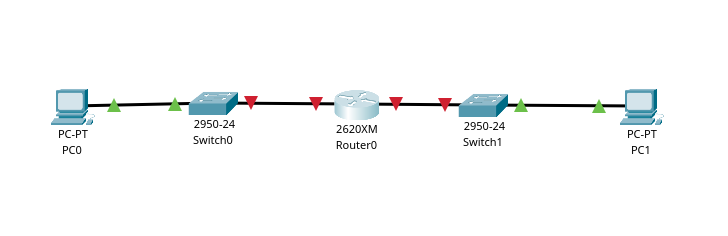
\includegraphics[width=1\textwidth]{img/1.png}
\end{figure}
\begin{figure}[h]
    \centering
    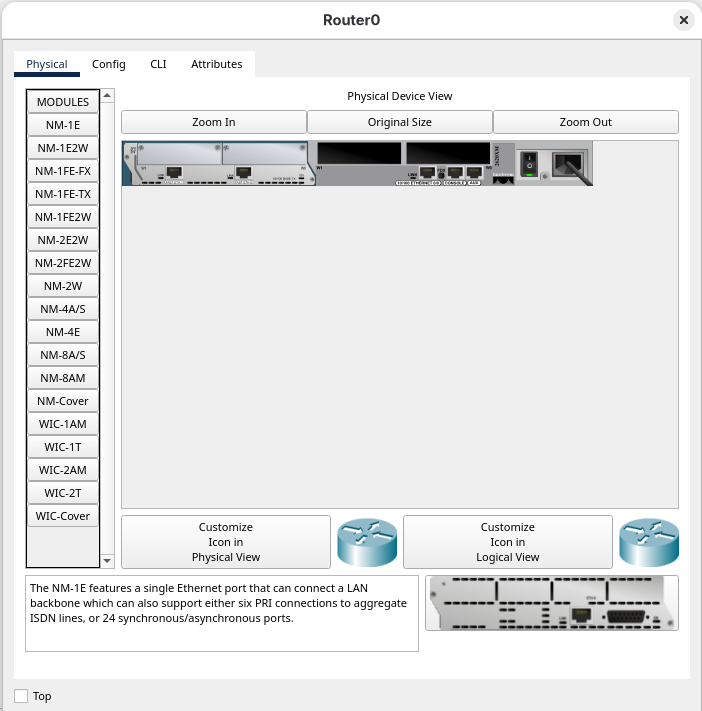
\includegraphics[width=1\textwidth]{img/2.png}
\end{figure}
\clearpage
در ادامه باید IP مسیریاب را تنظیم کنیم. پس با کلید بر روی مسیریاب و در بخش \lr{config}، \lr{FastEthernet1/x} را به صورت زیر پیکربندی می‌کنیم. پس از مشخص کردن مقدار \lr{IPv4} و \lr{subnetmask} مقدار \lr{Port status} را به on تغییر می‌دهیم.
\begin{figure}[h]
    \centering
    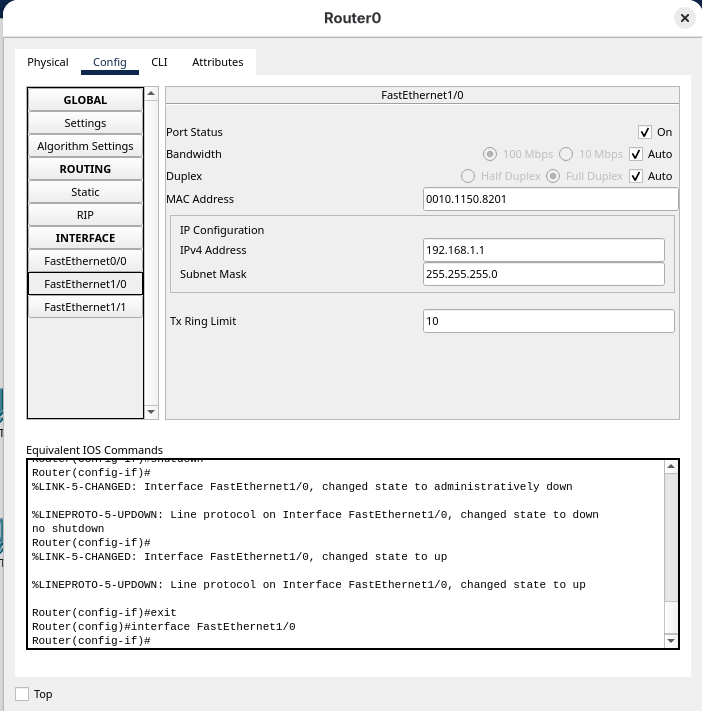
\includegraphics[width=1\textwidth]{img/3.png}
\end{figure}
\begin{figure}[h]
    \centering
    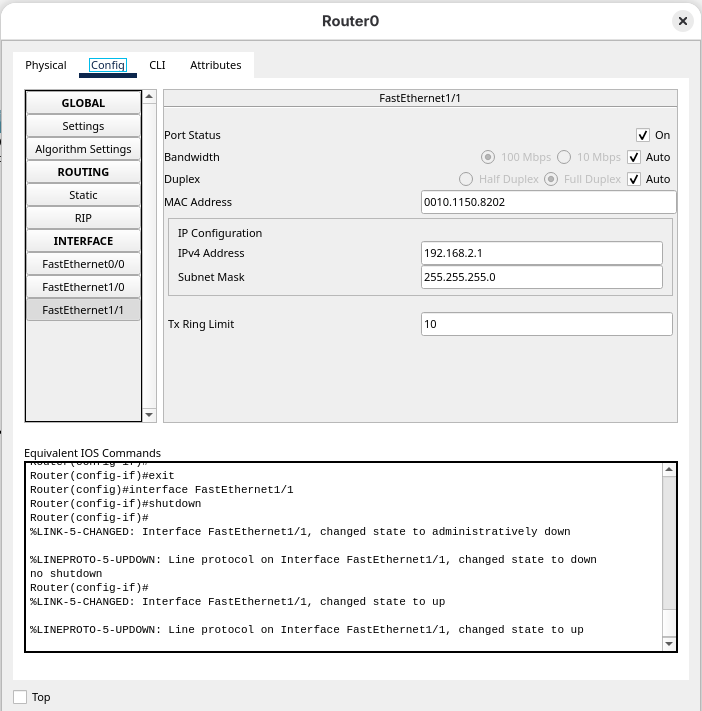
\includegraphics[width=1\textwidth]{img/4.png}
\end{figure}
و بعد از پیکربندی اتصال بین اجزا ایجاد می‌شود.
\begin{figure}[h]
    \centering
    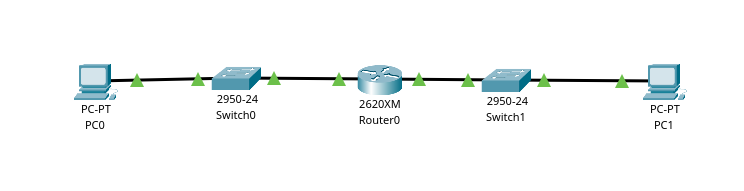
\includegraphics[width=1\textwidth]{img/5.png}
\end{figure}

\clearpage
جال باید کامپیوترها را نیز کانفیگ کنیم پس مانند قبل در تب \lr{config} ابتدا پیکربندی لازم را برای دستگاه انجام داده و بعد \lr{FastEthernet0} را تنظیم می‌کنیم.
\begin{figure}[h]
    \centering
    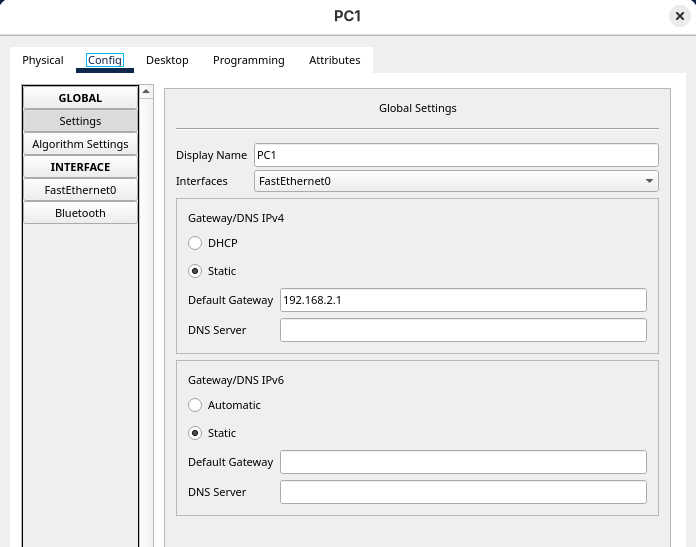
\includegraphics[width=0.70\textwidth]{img/6.png}
    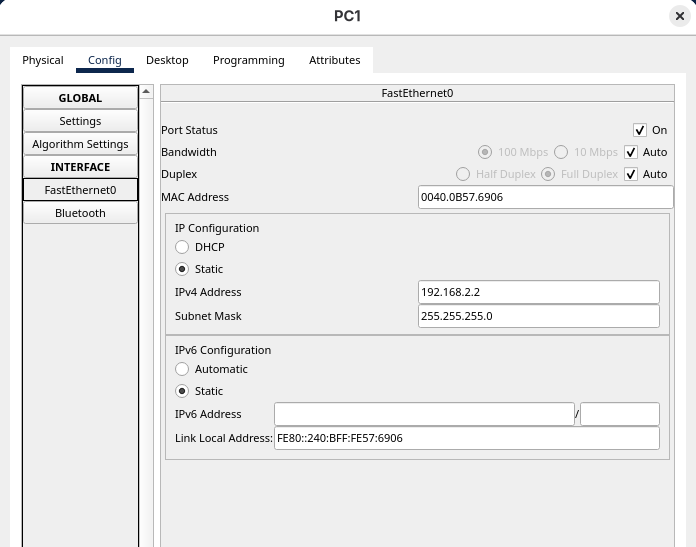
\includegraphics[width=0.8\textwidth]{img/7.png}
\end{figure}
\begin{figure}[h]
    \centering
\end{figure}
\begin{figure}[h]
    \centering
    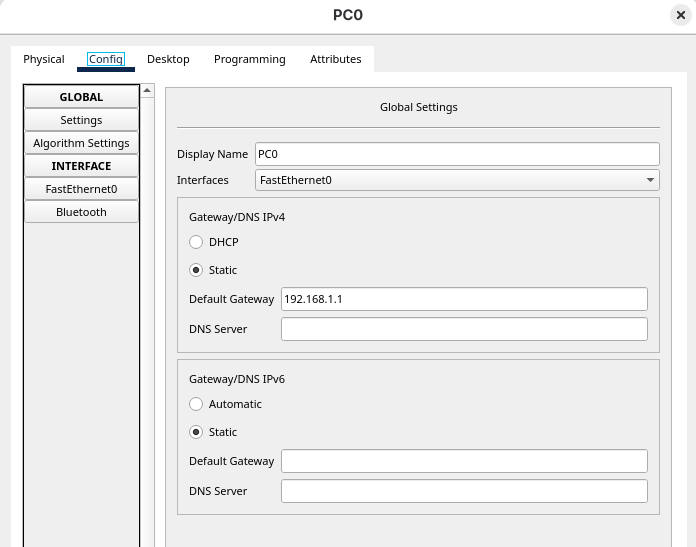
\includegraphics[width=0.8\textwidth]{img/8.png}
    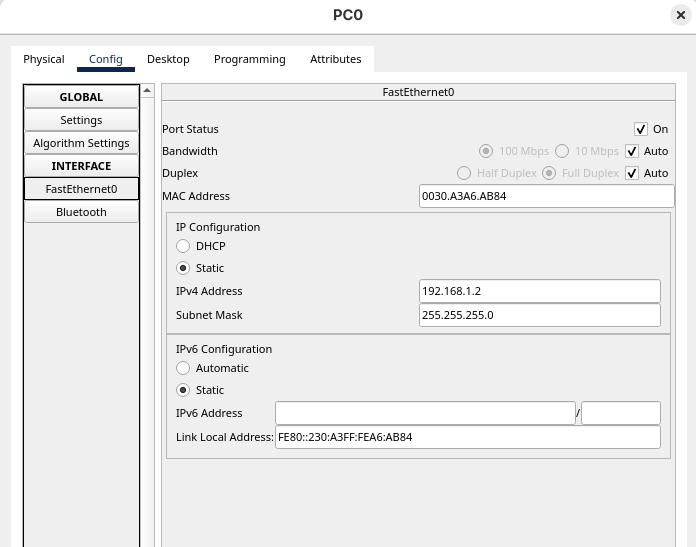
\includegraphics[width=0.8\textwidth]{img/9.png}
\end{figure}

\clearpage
برای تست کردن در کامپیوتر سمت چپ در بخش \lr{Desktop} در \lr{‫‪Command‬‬ Prompt‬‬} به کامپیوتر سمت راست پینگ می‌زنیم.

\begin{figure}[h]
    \centering
    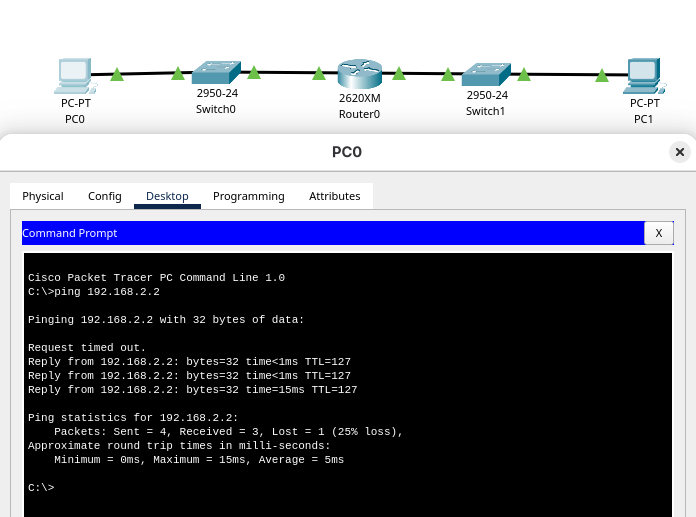
\includegraphics[width=1\textwidth]{img/10.png}
\end{figure}